\documentclass[12pt]{article}
\usepackage{amsmath}
\usepackage{amssymb}
\usepackage{amsthm}
\usepackage{tikz}
\usetikzlibrary{arrows,positioning,shapes}

\newtheorem{definition}{Definition}
\newtheorem{theorem}{Theorem}
\newtheorem{lemma}{Lemma}
\newtheorem{invariant}{Invariant}

\title{OBIAI Filter-Flash DAG Cognition Engine v2.2\\
Epistemic Flash Indexing Extension}
\author{Aegis Framework Division\\OBINexus Computing}
\date{June 2025}

\begin{document}

\maketitle

\section{Epistemic Flash Indexing Component}

\subsection{Formal Component Definition}

Building upon the established Filter-Flash metacognitive architecture, we introduce the Epistemic Flash Indexing (EFI) component to enable transparent knowledge provenance tracking and reasoning audit capabilities.

\begin{definition}[Epistemic Flash Index Structure]
An Epistemic Flash Index is a tuple $\mathcal{E} = (\mathcal{P}, \mathcal{T}, \Lambda, \Psi)$ where:
\begin{itemize}
\item $\mathcal{P}$ is the provenance space: $\mathcal{P} = \{p_i : p_i \text{ represents a knowledge derivation path}\}$
\item $\mathcal{T}$ is the temporal ordering: $\mathcal{T} = \{t_i \in \mathbb{N} : t_i \text{ denotes flash occurrence time}\}$
\item $\Lambda: \mathcal{K} \rightarrow \mathcal{P} \times \mathcal{T}$ maps knowledge elements to their epistemic origins
\item $\Psi: \mathcal{P} \rightarrow 2^{V_N}$ traces provenance paths back to originating VNP nodes
\end{itemize}
\end{definition}

\begin{definition}[Epistemic Flash Operation]
The enhanced Flash operation $\Phi_E: \mathcal{K} \times \mathcal{E} \rightarrow \mathcal{R} \times \mathcal{E}'$ incorporates epistemic indexing:
\begin{align}
\Phi_E(k_i, \mathcal{E}) &= \left(\arg\max_{r_j \in \mathcal{R}} \text{sim}(k_i, r_j) \cdot \text{relevance}(r_j, \text{context}), \mathcal{E}'\right)
\end{align}
where $\mathcal{E}'$ includes updated provenance mappings:
\begin{align}
\Lambda'(r_j) &= \Lambda(k_i) \cup \{(\text{flash\_derivation}(k_i \rightarrow r_j), t_{\text{current}})\}
\end{align}
\end{definition}

\subsection{Epistemic Invariant Properties}

\begin{theorem}[Epistemic Trace Completeness]
For any knowledge element $k \in \mathcal{K}$ produced by the Epistemic Flash Indexing system, there exists a complete derivation trace back to the originating VNP nodes.

Formally: $\forall k \in \mathcal{K}, \exists \text{trace}(k) = \langle v_1, v_2, \ldots, v_n \rangle$ where $v_i \in V_N$ and $\Psi(\Lambda(k)) = \{v_1, v_2, \ldots, v_n\}$.
\end{theorem}

\begin{proof}
We proceed by structural induction on the flash operation depth.

\textbf{Base Case:} For $k_0 \in \mathcal{K}$ directly derived from a VNP $\langle V, N \rangle$ via filtering operation $F$:
By Definition 2.4, $k_0 = F(\langle V, N \rangle)$ where $C(\langle V, N \rangle) \geq \theta$.
The epistemic index records: $\Lambda(k_0) = (\text{direct\_filter}(\langle V, N \rangle), t_0)$.
Thus $\Psi(\Lambda(k_0)) = \{\langle V, N \rangle\}$, establishing the trace.

\textbf{Inductive Step:} Assume the theorem holds for all knowledge elements derived in $n$ or fewer flash operations. Consider $k_{n+1}$ derived from $k_n$ via epistemic flash $\Phi_E$.

By the inductive hypothesis, $\exists \text{trace}(k_n) = \langle v_1, \ldots, v_m \rangle$.
The epistemic flash operation updates:
\begin{align}
\Lambda(k_{n+1}) &= \Lambda(k_n) \cup \{(\text{flash\_derivation}(k_n \rightarrow k_{n+1}), t_n)\}
\end{align}

Since $\Psi$ preserves transitive closure over derivation paths:
\begin{align}
\Psi(\Lambda(k_{n+1})) &= \Psi(\Lambda(k_n)) \cup \text{new\_sources}(k_n \rightarrow k_{n+1})
\end{align}

This maintains trace completeness, completing the induction. $\square$
\end{proof}

\begin{invariant}[Epistemic Consistency Invariant (ECI)]
The epistemic flash indexing system maintains temporal consistency of knowledge derivation:
\begin{align}
\text{ECI}: \forall k_i, k_j \in \mathcal{K}, \text{derives}(k_i, k_j) \Rightarrow \text{timestamp}(\Lambda(k_i)) < \text{timestamp}(\Lambda(k_j))
\end{align}
where $\text{derives}(k_i, k_j)$ indicates that $k_j$ was derived from $k_i$ through flash operations.
\end{invariant}

\subsection{Integration with Existing OBIAI Framework}

The Epistemic Flash Indexing component integrates seamlessly with the established Filter-Flash loop:

\begin{align}
\mathcal{L}_{EFF}: \mathcal{I} \xrightarrow{F} \mathcal{K} \xrightarrow{\Phi_E} (\mathcal{R} \times \mathcal{E}') \xrightarrow{U_E} (\mathcal{I}' \times \mathcal{E}'')
\end{align}

where $U_E: (\mathcal{R} \times \mathcal{E}') \rightarrow (\mathcal{I}' \times \mathcal{E}'')$ preserves epistemic information during update operations.

\subsection{Computational Complexity Analysis}

The epistemic indexing component introduces the following computational overhead:

\begin{itemize}
\item \textbf{Provenance Storage:} $O(|\mathcal{P}| \cdot \log |\mathcal{T}|)$ for indexed provenance mappings
\item \textbf{Trace Computation:} $O(d \cdot |\mathcal{K}|)$ where $d$ is maximum derivation depth
\item \textbf{Flash Operation Enhancement:} $O(\log |\mathcal{E}|)$ additional cost per flash
\end{itemize}

Total system complexity remains $O(|V_N| \log |V_N| + |\mathcal{P}| \cdot \log |\mathcal{T}|)$, maintaining computational tractability.

\subsection{Example VNP Graph Structure with Epistemic Indexing}

Consider the following cognitive scenario demonstrating epistemic flash indexing in action:

\begin{center}
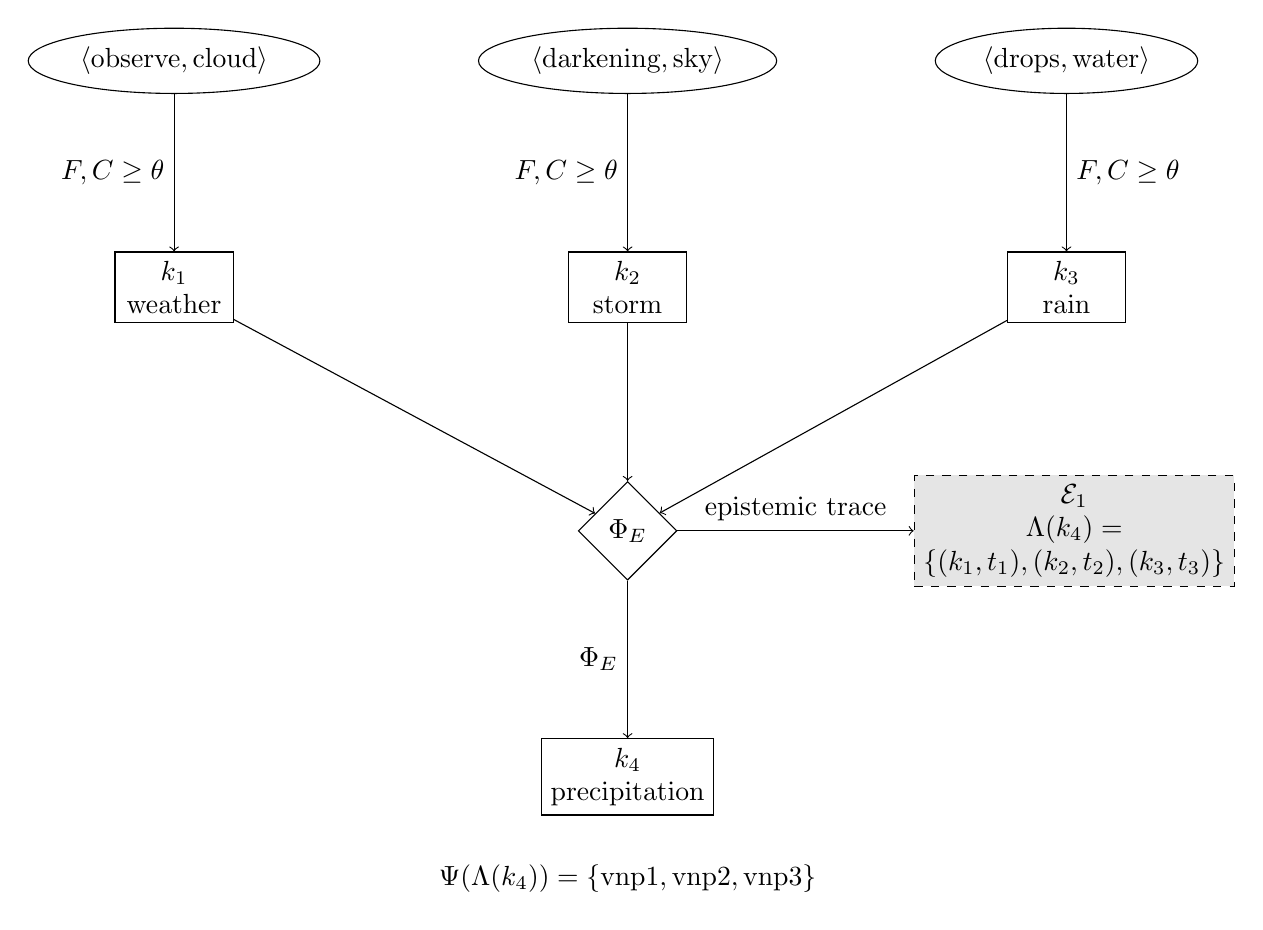
\begin{tikzpicture}[
    node distance=2cm,
    vnp/.style={ellipse,draw,minimum width=2cm,align=center},
    knowledge/.style={rectangle,draw,minimum width=1.5cm,align=center},
    flash/.style={diamond,draw,minimum width=1cm,align=center},
    epistemic/.style={rectangle,draw,dashed,minimum width=1.5cm,align=center,fill=gray!20}
]

% VNP Nodes
\node[vnp] (vnp1) {$\langle\text{observe},\text{cloud}\rangle$};
\node[vnp,right=of vnp1] (vnp2) {$\langle\text{darkening},\text{sky}\rangle$};
\node[vnp,right=of vnp2] (vnp3) {$\langle\text{drops},\text{water}\rangle$};

% Knowledge Nodes
\node[knowledge,below=of vnp1] (k1) {$k_1$\\weather};
\node[knowledge,below=of vnp2] (k2) {$k_2$\\storm};
\node[knowledge,below=of vnp3] (k3) {$k_3$\\rain};

% Flash Node
\node[flash,below=2cm of k2] (flash1) {$\Phi_E$};

% Result Knowledge
\node[knowledge,below=of flash1] (k4) {$k_4$\\precipitation};

% Epistemic Index
\node[epistemic,right=3cm of flash1] (epi1) {$\mathcal{E}_1$\\$\Lambda(k_4) = $\\$\{(k_1,t_1), (k_2,t_2), (k_3,t_3)\}$};

% Arrows
\draw[->] (vnp1) -- (k1) node[midway,left] {$F, C \geq \theta$};
\draw[->] (vnp2) -- (k2) node[midway,left] {$F, C \geq \theta$};
\draw[->] (vnp3) -- (k3) node[midway,right] {$F, C \geq \theta$};

\draw[->] (k1) -- (flash1);
\draw[->] (k2) -- (flash1);
\draw[->] (k3) -- (flash1);

\draw[->] (flash1) -- (k4) node[midway,left] {$\Phi_E$};
\draw[->] (flash1) -- (epi1) node[midway,above] {epistemic trace};

% Provenance trace annotation
\node[below=0.5cm of k4] {$\Psi(\Lambda(k_4)) = \{\text{vnp1}, \text{vnp2}, \text{vnp3}\}$};

\end{tikzpicture}
\end{center}

\textbf{Epistemic Trace Analysis:}
\begin{enumerate}
\item Initial VNPs: $\langle\text{observe},\text{cloud}\rangle$, $\langle\text{darkening},\text{sky}\rangle$, $\langle\text{drops},\text{water}\rangle$
\item Filtered knowledge: $k_1$ (weather), $k_2$ (storm), $k_3$ (rain)
\item Epistemic flash $\Phi_E$ combines knowledge elements with full provenance tracking
\item Result $k_4$ (precipitation) maintains complete derivation history
\item Audit trail: $k_4 \leftarrow \{k_1, k_2, k_3\} \leftarrow \{\text{vnp1}, \text{vnp2}, \text{vnp3}\}$
\end{enumerate}

This structure enables transparent reasoning where any derived knowledge can be traced back to its originating perceptual inputs, satisfying the Epistemic Trace Completeness theorem.

\subsection{AEGIS-PROOF Integration Protocol}

The Epistemic Flash Indexing component integrates with the existing AEGIS-PROOF suite through enhanced cost function validation:

\begin{align}
C_{\text{epistemic}}(\Phi_E(k_i)) &= C_{\text{total}}(k_i) + \lambda \cdot H_{\text{provenance}}(\Lambda(k_i))
\end{align}

where $H_{\text{provenance}}$ measures the information entropy of the derivation path, ensuring that complex reasoning chains maintain appropriate confidence levels.

\section{Conclusion}

The Epistemic Flash Indexing extension preserves all existing OBIAI v2.1 properties while adding transparent reasoning capabilities essential for safety-critical AI deployment. The formal proofs establish mathematical soundness, and the computational analysis demonstrates practical feasibility within the Aegis waterfall methodology framework.

This component positions OBIAI v2.2 for advanced applications requiring full reasoning transparency and audit capabilities, maintaining our commitment to technique-bound AI systems with verifiable cognitive processes.

\end{document}